\documentclass[output=paper]{LSP/langsci} 
\ChapterDOI{10.5281/zenodo.1090944}

\title{Predicting cognate translation}
\author{Silvia Hansen-Schirra\and 
Jean Nitzke\lastand
Katharina Oster\affiliation{FTSK Germersheim, Johannes-Gutenberg-Universtität Mainz}}

\abstract{Empirically-based translation research has so far been developed within two major self-standing approaches: corpus-based work on properties of translated texts or translation universals (product) and experimental studies of translators’ expert performance (process). Recently, advances in corpus architecture and multi-level corpus querying are combined with methods from psycholinguistics and cognitive science in order to determine predictors for translation candidate probabilities, which in turn may range from free to literal translation solutions. In the corpus-based realm, free translations lead to normalization effects, whereas literal ones trigger shining-through. Speaking from a cognitive point of view, shining-through can be related to the literal translation hypothesis, while normalization may occur due to monitoring processes.

This paper investigates the conditions under which cognates are translated into more literal or free translation candidates. Some of the influential factors are text internal (e.g. context) or external (e.g. language status); others are translation inherent, such as the expertise of the translator and the translation mode. The former are discussed from a product-based perspective, the latter are analyzed in a more process-oriented manner. Multi-method approaches including translation corpora and experimental data are used for predicting the probability of cognate variation in translation. As a consequence, the predictors are discussed against the background of the monitor model.}

\maketitle
\begin{document}

\section{Cognition meets translation constraints}\label{hansenschirraetal:sec:1}
\citet{Toury1995} identifies two laws of translational behavior: he explains that there is a law of growing standardization, i.e., that ``in translation, textual relations obtaining in the original are often modified, sometimes to the point of being totally ignored, in favour of (more) habitual options offered by a target repertoire” \citep[268]{Toury1995}. However, Toury also suggests that translators tend to produce a translated utterance not by retrieving the \isi{target language} via their own linguistic knowledge, but directly from the source utterance itself. The universality of discourse transfer is expressed through another translational law, the law of interference: ``in translation, phenomena pertaining to the make-up of the source text tend to be transferred to the target text'' \citep[275]{Toury1995}.
 
From a corpus-based perspective, the first law is also reflected in \citet{Baker1996} universal feature of normalization: Normalization (or conservatism) means that translators tend to conform to the typical patterns of the \isi{target language} or even to exaggerate their use. This universal feature also includes the tendency to normalize marked and ungrammatical structures. But if the status of the \isi{source language} is significantly higher than the status of the \isi{target language} (for example, English compared with other languages in the field of software), normalization in translations is weakened or the opposite tendency might even be observed. If this is the case, the typical patterns of the \isi{source language} are still visible in the translations, which \citet{Teich2003} calls shining-through.

The continuum between foreignization and domestication is also reflected in the choice of literal vs. more or less free translation strategies and procedures as well as formal vs. dynamic equivalence \citep{VinayDarbelnet1995, Newmark1988}. However, \citet{TirkonnenCondit2005} argues that \isi{literal translation} is a default \isi{translation procedure}, which is cognitively preferred to others. \citet{Chesterman2011} and \citet{Halverson2015} reintroduce the concept of \isi{literal translation}, assuming that entrenchment effects strengthen the \isi{co-activation} of linguistic patterns and thus reduce the \isi{cognitive load} during translation for literal renderings (see \citet{SchaefferCarl2014} for an empirical operationalization).

From a cognitive perspective, \isi{literal translation} can be explained by the priming effect. When a translator reads a source text element, a specific element in the \isi{target language} is primed due to close memory links. It can then be more easily produced than other translation solutions. These close memory links might exist on different linguistic levels. Elements of similar form, similar \isi{word class} and similar meaning have strong links across language borders.

The \isi{monitor model} was proposed by \citet{TirkkonenCondit2005}. She assumes that translators follow a predefined translation root, which is the easiest way to translate a text. But they constantly \isi{monitor} production and as soon as a problem is encountered in this default translation root, they stop the \isi{literal translation} process and try to find a better solution. This model has been tested by \citet{CarlDragsted2012}.

The continuum between monitoring and priming/\isi{literal translation} could be another way to perceive Toury's laws of standardization and interference. The \isi{monitor model}, however, still exhibits some shortcomings. It is, for example, not precise enough to determine which factors influence priming. As priming might exist on several linguistic levels, what determines its strength? Finding answers to these questions and thus creating a more elaborate \isi{monitor model} could help to predict translational behavior.

For this purpose, we will investigate cognates (translation equivalents which share a similar form). Several studies have shown that the number of cognates in translations varies significantly depending on other factors such as language status of the respective languages \citep{VintarHansenSchirra2005} and translation mode \citepv{Oster}. Cognates are relatively easy to manage in experimental settings and can be investigated in many language pairs. We thus believe that they are a good basis for the investigation of the different priming roots.

In the following, we will examine different factors that might influence the production of cognates. Some are text internal, such as context or external such as language status of the respective languages, as well as historical developments. These constraints will be investigated from a product-based perspective. However, other factors are translation inherent, such as the expertise of the translator and the translation mode, which will be analyzed from a more process-oriented perspective. We will show how the translation of cognates can be predicted within the context of the different constraints and finally discuss how the predictors can be implemented into the \isi{monitor model}.

\section{Cultural-political predictors}\label{hansenschirraetal:sec:2}
Our hypothesis is that cultural-political predictors influence translation choices. In the following, we introduce two external factors that predict translation behavior: language status and socio-historical influences.

\subsection{Language status}\label{hansenschirraetal:sec:2.1}
The first study deals with two language pairs for which we assume that the relation between the source and target languages and cultures differ: English-\ili{German} and English-\ili{Slovene}. Since 1945, \ili{German} has seemed to be susceptible to influences from the English language \citep{Carstensen1965}. In contrast, \ili{Slovene} is less influenced and exhibits language protectionism on a political level \citep{VintarHansenSchirra2005}.

The results discussed here were published in \citet{VintarHansenSchirra2005}, which includes English-\ili{German} and English-\ili{Slovene} translations as well as \ili{German} and \ili{Slovene} original comparable texts. The authors fully automatically extracted the \isi{cognate} pairs from the parallel corpora compiled for the study from popular scientific texts using an implementation of the Levenshtein's edit distance algorithm in the Perl String::Approx module (for details see ibid.). The original comparable texts were used as a tertium comparationis for the \isi{cognate} frequencies.

For the comparison of the \isi{cognate} frequencies, a parallel English-\ili{German} and English-\ili{Slovene} subcorpus and a comparable \ili{German} and \ili{Slovene} subcorpus were created. These had to be as comparable as possible in terms of corpus size and register. For this reason, all subcorpora comprised 10,000 tokens of popular scientific texts. Following \citet{Biber1995}, each subcorpus was composed of ten text samples consisting of roughly 1000 tokens. This guarantees that the sub-corpora is as well-balanced as possible. The COSMAS corpus was used as a monolingual reference corpora for \ili{German}, and the FIDA was used for \ili{Slovene} \citep{VintarHansenSchirra2005}.

The comparison of the \isi{cognate} frequencies in \ili{Slovene} and \ili{German} translations and \ili{Slovene} and \ili{German} originals shows that, in general, \ili{German} has more cognates than \ili{Slovene}, and more specifically \ili{German} translations exhibit the highest \isi{cognate} frequency (see \ref{hansenschirraetal:tab:1}; $\chi^{2}=60.33, df= 1, p>.001$).

\begin{table}
\caption{Cognate frequencies normalized to a corpus size of 10,000 words}
\label{hansenschirraetal:tab:1}
\begin{tabularx}{\textwidth}{XXX}
\lsptoprule
            &  {Slovene}    &  {German}    \\ \midrule
Original    & 254       & 356       \\
Translation & 189       & 652       \\
\lspbottomrule
\end{tabularx}
\end{table}

\newpage 
These results illustrate that \ili{German} is more susceptible to \isi{cognate} use than \ili{Slovene}, and this is even more prominent in translations. However, a contrary tendency can be observed for \ili{Slovene} translations which have fewer cognates than \ili{Slovene} original texts. This might be interpreted as a slight aversion towards the use of cognates in \ili{Slovene} translations.

On the one hand, it can be said that the context of a word is very important for the choice between \isi{cognate} and native word. For instance, the English word \textit{action} was not only translated with its \ili{Slovene} \isi{cognate} \textit{akcija}, but a series of non-\isi{cognate} translations (\textit{delovanje, tehnika, ukrepanje, aktivnost, izvedba, operacija, udejstvovanje}) could also be found in the corpus depending on the context of the word. On the other hand, repetitions in translations are avoided by using the \isi{cognate} as well as the native words for stylistic purposes (e.g. English \textit{volcanic activity}, \ili{German} \textit{vulkanische Aktivität}, \textit{vulkanische Tätigkeit}, \textit{vulkanische Ausbrüche},\textit{ vulkanische Bewegung}).

Nevertheless, it seems that \ili{German} is more receptive to the use of cognates than \ili{Slovene}. The preference of cognates in \ili{German} might be explained by two different tendencies: first, it might mirror the use of Anglicisms in \ili{German}, which in turn reflects the strong influence English nowadays has on the \ili{German} language (especially as lingua franca of science, \citealt{Ammon2001}). On the other hand, the \isi{cognate} use might be an indicator of the susceptibility of the \ili{German} language towards internationalisms rooted in a common etymological history \citep{Braunetal2003}. In contrast, it might be the case that \ili{Slovene} as a `minor language' tries to avoid foreign language material by using only native words to protect itself from language change. The tendency for or against cognates might therefore be related to the overall language – and translation – policy in the target society. Thus, avoiding cognates might be a strategy of linguistic purism and protectionism. 

\subsubsection{Socio-historical influences}
\label{hansenschirraetal:sec:2.2}

Social-historical factors might influence the use of cognates, as well. In the following, we will compare the development of cognates in different languages over the course of time with a bottom-up methodology using the Google Books \textit{Ngram Viewer}.\footnote{https://books.google.com/ngrams, last accessed 13th August 2016} This tool shows the frequency of words and phrases used in the selected book corpora and over the course of the selected years (between 1500 and 2008).


\begin{figure}
\caption{Diachronic development of \textit{technology} and its cognate versions in German, Spanish, Italian, and French from 1900 to 2008.}
\label{hansenschirraetal:fig:1}
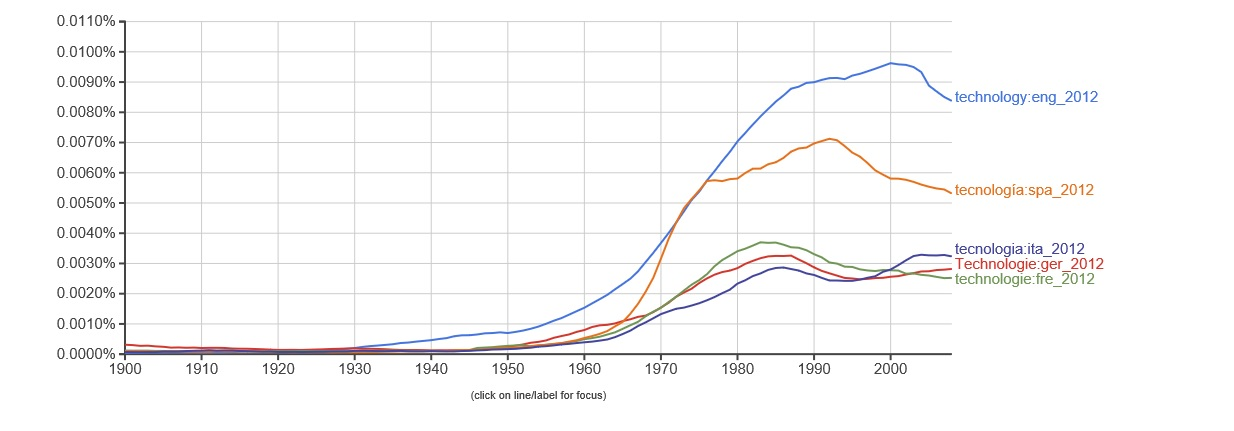
\includegraphics[width=\textwidth]{figures/hansen-schirra/HansenSchirra1.jpg}
\end{figure}

\begin{figure}
\caption{Diachronic development of \textit{international} and its cognate versions in German, Spanish, Italian, and French from 1900 to 2008.}
\label{hansenschirraetal:fig:2}
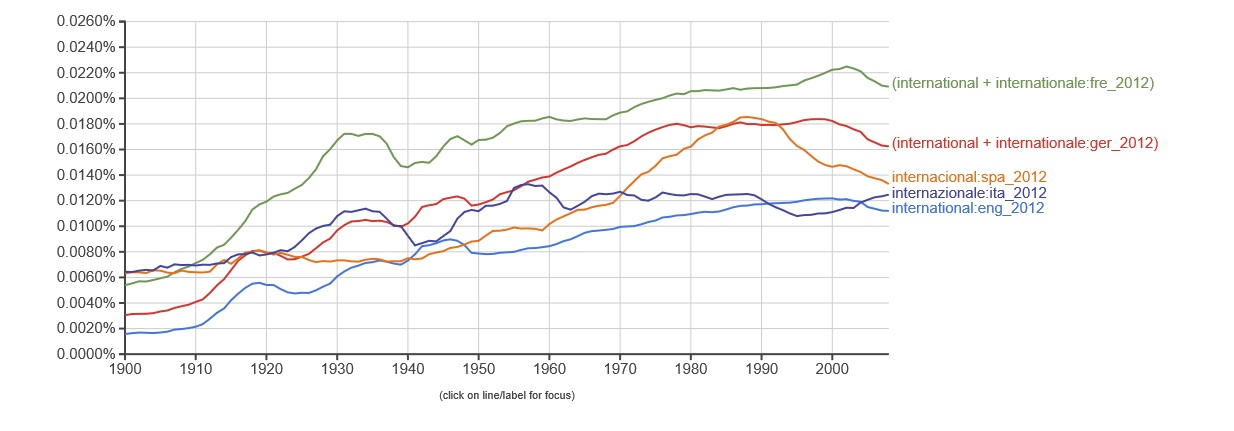
\includegraphics[width=\textwidth]{figures/hansen-schirra/HansenSchirra2.jpg}
\end{figure}

\begin{figure}
\caption{Diachronic development of \textit{globalization (globalisation)} and its cognate versions in German, Spanish, Italian, and French from 1950 to 2008.}
\label{hansenschirraetal:fig:3}
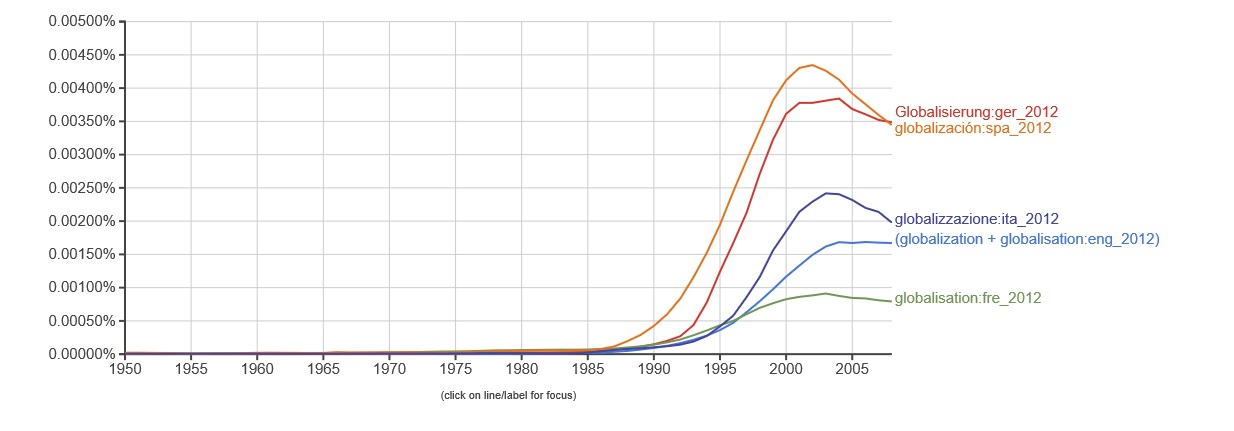
\includegraphics[width=\textwidth]{figures/hansen-schirra/HansenSchirra3.jpg}
\end{figure}


\clearpage  

\begin{figure}
\caption{Diachronic development of \textit{tariff} and its cognate versions in German, Spanish, Italian, and French from 1900 to 2008.}
\label{hansenschirraetal:fig:4}
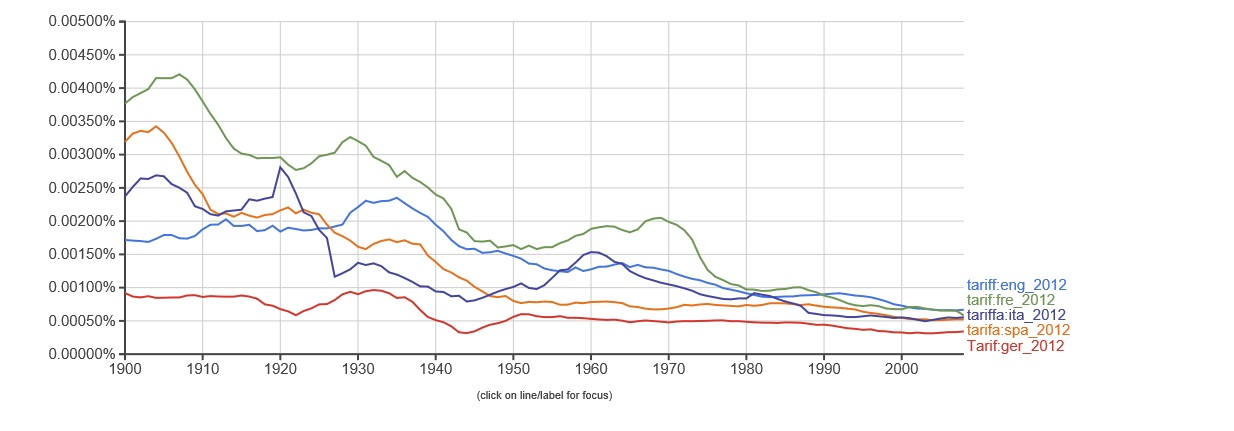
\includegraphics[width=\textwidth]{figures/hansen-schirra/HansenSchirra4.jpg}
\end{figure}


Figures \ref{hansenschirraetal:fig:1}-\ref{hansenschirraetal:fig:4} show the diachronic development of four \isi{cognate} words in five different languages (English, \ili{French}, \ili{German}, \ili{Italian}, \ili{Spanish}) from 1900 to 2008 (apart from \textit{globalization} – \figref{hansenschirraetal:fig:3} – because the word did not occur in the first half of the 20\textsuperscript{th} century). All figures show similar developments of the presented words in the different languages over the course of time.



\textit{Technology} and its multilingual \isi{cognate} representations (\figref{hansenschirraetal:fig:1}) hardly occurred in the corpora before the mid-60s, when the frequency of the words started to increase rapidly for the next decades. Although the term \textit{technology} has existed since 1910 in the English language and originates from the Greek \textit{tekhnologia}, the term \textit{high technology} was coined only in 1964, which might also characterize the beginning of this linguistic development.\footnote{\url{http://www.etymonline.com/index.php?allowed_in_frame=0&search=technology}, last accessed 13th August 2016}

The use of \textit{international} and its multilingual \isi{cognate} representations (\figref{hansenschirraetal:fig:2}) increases steadily, but is not bound to a specific date or event. This indicates that international relations and economics – well known social developments – have become more important in our societies in the last century and hence affected the languages as well. In contrast to \textit{technology}, \textit{international} has English roots and was coined by the English social philosopher and solicitor J. Bentham.\footnote{\url{http://www.duden.de/rechtschreibung/international} and \url{http://www.etymonline.com/index.php?allowed_in_frame=0&search=international}, last accessed 13th August 2016} However, the components of \textit{international} (\textit{inter}\footnote{\url{http://www.duden.de/rechtschreibung/inter_}, last accessed 13th August 2016} and \textit{national}\footnote{\url{http://dwds.de/?view=1\&qu=national}, last accessed 13th August 2016}) have \ili{Latin} roots, a language that influenced all examined languages. Hence, this might have promoted the inclusion and acceptance of the English word in the other languages.

\newpage 
\textit{Globalization} and its equivalents (\figref{hansenschirraetal:fig:3}) show a similar development to \textit{technology}, but the increase is more rapid and much later. The word globalization only emerged in 1961, although the verb \textit{globalize} was first recorded in 1953, but not in the sense that refers to global economic systems.\footnote{\url{http://www.etymonline.com/index.php?term=globalize&allowed_in_frame=0}, last accessed 13th August 2016} Here, we can observe an interesting finding since the \ili{German} and \ili{Spanish} cognates appeared more frequently and earlier in time. This development cannot be attributed to the influence of English as lingua franca but rather to the fact that this internationalism derived from the \ili{Latin} word “globus”. This clearly shows that common etymological roots might trigger \isi{cognate} usage as well.

In contrast to the other example, the use of \textit{tariff} and its cognates decreases in the last decade in all five languages, albeit to different degrees. This might be caused by a restriction of meaning because the word \textit{tariff} used to have an extended meaning, namely “prices” in general, whereas today it is mainly used within the context of taxes and wages.\footnote{\url{http://dwds.de/?qu=Tarif}, last accessed 13th August 2016} 

The examples discussed here indicate that the usage of cognates varies according to societal and technological development. The word might have popped up in one language, but due to common language roots it might be more easily accepted in other languages as well. Furthermore, language change, like extending or narrowing down the meaning of a word may also have an influence \citep{Koselleck1979}.

\section{Linguistic predictors} \label{hansenschirraetal:sec:3}
\subsection{Linguistic context} \label{hansenschirraetal:sec:3.1}
The context, in which the words are embedded, is a very important factor for translation and translation choices – a phenomenon also known as intra-lingual communication. A \textit{table} can, for example, be either furniture or a chart and the context in which the word is used usually clearly specifies which table is meant. We hypothesize that cognates are more frequently translated with a \isi{cognate} when the translators are asked to translate a single word than when the \isi{cognate} is integrated in a complete text. 

To test this hypothesis, we ran a study with 67 participants, who had to translate single words in a list (with information on the \isi{word class}) and a complete text that contained numerous cognates.\footnote{The experiments in Section \ref{hansenschirraetal:sec:3.1} and \ref{hansenschirraetal:sec:4.1} were carried out at the \textsc{ftsk}. Translation students participated during a lecture in the different experiments. Since the experiments were part of their course, they did not receive any further credit for participation. The participants were informed that the results were treated anonymously and that they were only used for scientific purposes. The students were further informed that their participation had no influence on their grades and that they could withdraw from the experiment at any time.} Both settings contained the same cognates. For the study, two political texts were chosen (190 and 186 words, respectively). A total of 20 cognates were isolated in each text and used to compose the \isi{cognate} list. The participants were \ili{German} native speakers who studied English and translation and were asked to translate one word list and one text. In addition, we set a time limit of three minutes for the list and 14 minutes for the texts, because we wanted the participants to first prepare a translation draft to ensure that they used the words first activated in their \isi{mental lexicon}. The results are presented in Table 2.\footnote{Thanks to Jan Skawski and Kai Schuhmacher who conducted the experiment and came up with first results in the context of a seminar paper.}

\begin{table}
\caption{Percentage of translations with cognates, with non-cognates, or no translation at all depending on an existing context}
\label{hansenschirraetal:tab:2}
\begin{tabularx}{\linewidth}{XXXX}
\lsptoprule
                & Cognate   & non-\isi{cognate}   & no translation    \\ \midrule
without context & 57,39     & 32,24         & 10,37             \\
with context    & 37,27     & 54,91         & 7,82              \\ 
\lspbottomrule
\end{tabularx}
\end{table}

While cognates in the list are translated as cognates in over 57\% of the cases, they were only translated with cognates in around 37\% when they were presented in context. The picture is reversed for non-cognates translations (32\% without context, 55\% with context). In some instances, the translators were not able to produce a translation or chose to omit the word in the target text.

\begin{figure}
\begin{tikzpicture}
        \begin{axis}[
            width = .8\textwidth,
            hide x axis,
            axis lines*=left,  
            enlarge x limits = false
   		]
        \addplot+[only marks, mark options = {scale=1.2,fill=lsMidBlue, draw=lsMidBlue}] plot coordinates {(1,-65.61935484) (2,-62.39354839) (3,-55.55555556) (4,-51.11935484) (5,-44.66774194) (6,-42.91111111) (7,-40.9483871) (8,-40.66111111) (9,-40.66111111) (10,-40.6483871) (11,-33.8888889) (12,-32.77777778) (13,-28.11290323) (14,-27.74516129) (15,-27.22222222) (16,-27.22222222) (17,-27.12258065) (18,-26.46451613) (19,-25.1483871) (20,-23.88888889) (21,-18.96666667) (22,-17.6) (23,-14.84193548) (24,-13.88888889) (25,-9.866666667) (26,-9.677419355) (27,-4.706451613) (28,-4.444444444) (29,-3.544444444) (30,0) (31,0) (32,0.551612903) (33,0.987096774) (34,1.533333333) (35,4.444444444) (36,6.322222222) (37,8.333333333) (38,9.1) (39,17.6) (40,23.07419355)};
        \addplot+[mark=,black, /tikz/densely dashed] plot coordinates {(0,0) (40,0)};
        \end{axis}
    \end{tikzpicture}
%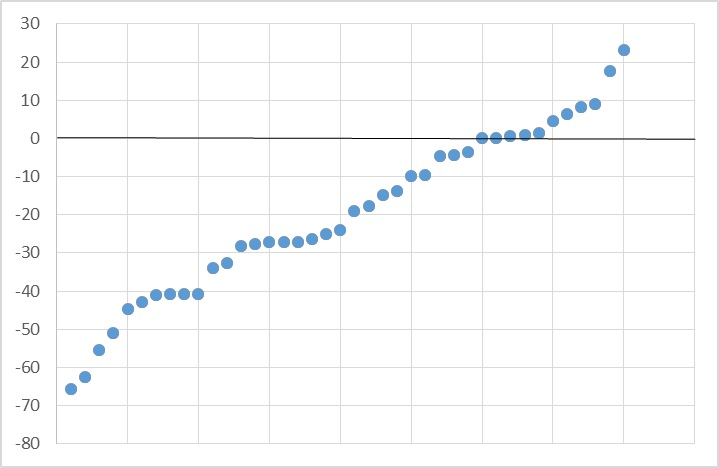
\includegraphics[width=0.7\textwidth]{figures/hansen-schirra/HansenSchirra5.jpg}
\caption{Distribution of decline (below zero) and increase (above zero) of cognate translation with context.}
\label{hansenschirraetal:fig:5}
\end{figure}

If we compare the translations of the same word with and without context, different patterns can be observed: Some words were translated by most participants with a \isi{cognate} in the list condition, but were translated less often with a \isi{cognate} in the text condition. For example, \textit{priorities} was translated with a \isi{cognate} in 93.6\% of cases when it was only presented as a single word, or it was not translated at all (no participant translated the word with a non-\isi{cognate}). In the text condition, however, \textit{priorities} was translated as a \isi{cognate} in only 52.9~\% of cases, and 41.2~\% of the participants chose a non-\isi{cognate translation}. As another example, \textit{shield} was mainly translated as a \isi{cognate} (80.6~\%) in the list condition and never as a non-\isi{cognate}, but it was only translated as a \isi{cognate} in a quarter of the cases in the condition with context and as a non-\isi{cognate} in 60~\%. A point in \figref{hansenschirraetal:fig:5} represents one word of our texts/lists and the ratio of its decrease or increase (in percent) when translated in context compared to the single \isi{word translation}. There were also instances for which it was the other way around (see \figref{hansenschirraetal:fig:5} and \ref{hansenschirraetal:fig:6}). For example, \textit{diversity} was hardly translated with its \isi{cognate} in the list task (3.6\%), but the frequency increased considerably in the text task (26.3\%). However, this is rather the exception than the rule, as can be seen in \figref{hansenschirraetal:fig:6}, which shows how often the \isi{cognate} use radically increased ($>10\%$), only slightly changed ($\pm 10\%$), or radically decreased ($>10\%$).

\begin{figure}

\begin{tikzpicture}
        \begin{axis}[
            width  = .8\textwidth,
            height = .3\textheight, 
            symbolic y coords={radical increase, minor changes, radical decrease},
            axis lines*=left,  
            bar width = 15pt,
            axis on top,
            xmajorgrids, tick align=inside,
            major grid style={draw=white},
            xbar stacked,
            xmin=0,
            xmax=70,
    		ytick=data,
			enlarge x limits = false
        ]
        \addplot+[lsMidBlue] plot coordinates {(5,radical decrease) (30,minor changes) (65,radical increase)};
        \end{axis}
    \end{tikzpicture}
%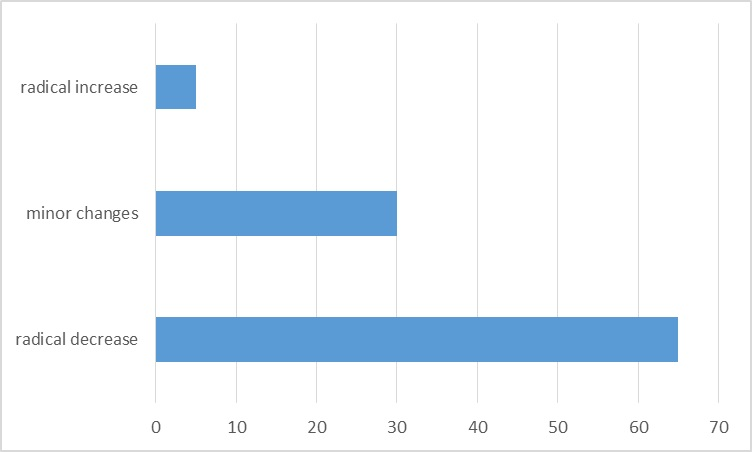
\includegraphics[width=0.7\textwidth]{figures/hansen-schirra/HansenSchirra6.jpg}
\caption{Change in translation strategy with context in percentage}
\label{hansenschirraetal:fig:6}
\end{figure} 

The analysis shows that the use of cognates in translations is dependent on the context of the translation. In general, the participants chose a \isi{cognate} less frequently, when they were translating a whole text than when they only had to find \ili{German} equivalents in a word list. This might indicate that the \isi{cognate translation} is the ``safest'' without context, because the \isi{cognate} is not only similar in meaning, but also in form. When a \isi{cognate} is embedded in context, however, the translators are more secure about which translation choice to select.

\subsection{Text type}\label{hansenschirraetal:sec:3.2}
As shown in the preceding section, context has an influence on \isi{cognate} use. But why would e.g. \textit{diversity }be translated more often as a \isi{cognate} in a political text than in a list of single words? We assume that this behavior was triggered by the text type. Maybe the participants thought that the use of the \isi{cognate translation} is more natural in the political context, although they are aware of a non-\isi{cognate} alternative. Hence, we hypothesize that text types influence the use of cognates.

In the following, we used the statistics component of the online tool \textit{DWDS}\footnote{„Digitales Wörterbuch der deutschen Sprache“ (Digital Dictionary of the \ili{German} language), \url{www.dwds.de}} to observe the intralingual influence of different text types on the use of cognates. We used the following pairs of cognates and non-cognates, and compared them for two different text types, namely newspapers (\textsc{np}) vs. academic texts (\textsc{at}). We chose the following example because we assumed that they might be used differently in the two text types. Further, we wanted to cover different word classes\footnote{We chose the most frequent non-cognates of the translation test in Section \ref{hansenschirraetal:sec:3.1} to come up with these pairs. We neglected translations which only occurred once or twice.}:

\begin{itemize}
\item \textit{komplex} (\isi{cognate}), \textit{kompliziert }(\isi{cognate}) vs. \textit{schwierig} (non-\isi{cognate})
\item \textit{original} (\isi{cognate}) vs. \textit{echt} (non-\isi{cognate})
\item \textit{publizieren/ Publikation} (\isi{cognate}) vs. \textit{veröffentlichen/Veröffentlichung} (non-\isi{cognate})
\item \textit{Maschine} (\isi{cognate}), \textit{Apparat} (\isi{cognate}) vs. \textit{Gerät} (non-\isi{cognate})
\item \textit{spezifisch} (\isi{cognate}), \textit{charakteristisch} (\isi{cognate}), \textit{typisch} (\isi{cognate}) vs. \textit{besonders} (non-\isi{cognate}), \textit{deutlich} (non-\isi{cognate})
\end{itemize}


The results in \figref{hansenschirraetal:fig:7} show that, in general, there is no clear preference for cognates or non-cognates. However, when comparing different text types, we can see that cognates are preferred in academic texts compared to newspapers for the same \isi{cognate}/non-\isi{cognate} pair. This holds true for all our examples displayed in \figref{hansenschirraetal:fig:7}, although the difference for the pair \textit{komplex}, \textit{kompliziert} (cognates) vs. \textit{schwierig} (non-\isi{cognate}) is only very small. 

The interpretation of these results may be twofold: 

First, it is possible to assume that \ili{German} academic writing might be influenced by the lingua franca of science, which is English \citep{Ammon2001}. Language contact might result in a higher frequency of Anglicisms, internationalisms and cognates in \ili{German} academic writing. In addition, academic texts convey a high frequency of technical terms such as Latinisms, Grecisms and Anglicisms \citep{Braunetal2003}. At same time, these are the roots of cognates because they have typically been introduced into and established in different languages and language families.

\begin{figure}
%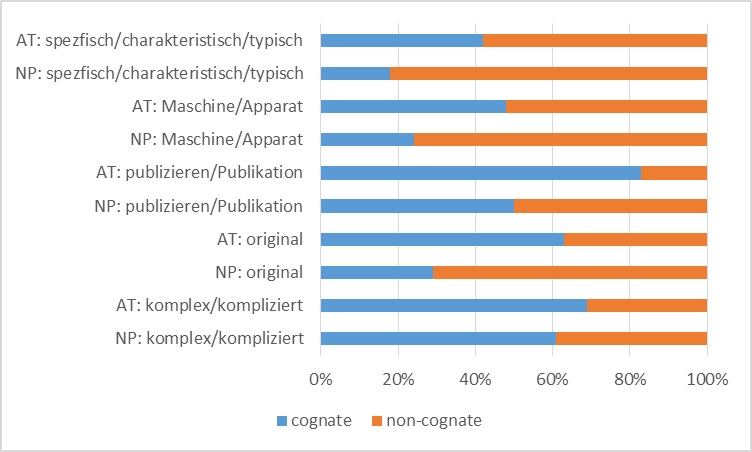
\includegraphics[width=\textwidth]{figures/hansen-schirra/HansenSchirra7.jpg}
	\resizebox{\textwidth}{!}{
	\begin{tikzpicture}
        \begin{axis}[
            width  = \textwidth,
            %height = .4\textheight, 
            symbolic y coords={{AT: spezifisch/charakteristisch/typisch}, {NP: spezifisch/charakteristisch/typisch}, {AT: Maschine/Apparat}, {NP: Maschine/Apparat}, {AT: publizieren/Publikation}, {NP: publizieren/Publikation}, {AT: original}, {NP: original}, {AT: komplex/kompliziert}, {NP: komplex/kompliziert}},
            axis lines*=left,  
            bar width = 18pt,
            axis on top,
            xmajorgrids, tick align=inside,
            major grid style={draw=white},
            xbar stacked,
            xmax=100,
            xmin=0,
    		legend style={at={(0.5,-0.1)}, anchor=north,legend columns=-1},
    		ytick=data,
        ]
        \addplot+[lsMidBlue] plot coordinates {(42,AT: spezifisch/charakteristisch/typisch) (18,NP: spezifisch/charakteristisch/typisch) (48,AT: Maschine/Apparat) (24,NP: Maschine/Apparat) (83,AT: publizieren/Publikation) (50,NP: publizieren/Publikation) (63,AT: original) (29,NP: original) (69,AT: komplex/kompliziert) (61,NP: komplex/kompliziert)};
		\addplot+[lsMidOrange] plot coordinates {(58,AT: spezifisch/charakteristisch/typisch) (82,NP: spezifisch/charakteristisch/typisch) (52,AT: Maschine/Apparat) (76,NP: Maschine/Apparat) (17,AT: publizieren/Publikation) (50,NP: publizieren/Publikation) (37,AT: original) (71,NP: original) (31,AT: komplex/kompliziert) (39,NP: komplex/kompliziert)};
    	\legend{\isi{cognate}, non-cognate}
        \end{axis}
    \end{tikzpicture}}
\caption{Examples for cognates and non-cognates in academic texts (AT) vs. newspapers (NP)}
\label{hansenschirraetal:fig:7}
\end{figure}

\newpage 
Secondly, the preference for non-cognates in newspaper texts might reflect a protectionary strategy of journalists towards their own language. They try to avoid cognates, which commonly have their routes in foreign languages, in favor of \ili{German} synonyms \citep{Liesem2014}. At the same time, shining-through effects of English constructions or internationalisms can also be found in popular-scientific texts translated from English to \ili{German} \citep{HansenSchirraetal2012} conveying a certain degree of technicality, which might be comparable to the academic text type under investigation.

In summary, typical preferences in terms of \isi{cognate} usage can be identified for different text types. Further, we assume that a more in depth study might complete the picture. It seems, for example, reasonable that legal or technical texts – or in general very domain-specific texts – contain more cognates than newspaper texts or other general language texts.

\section{Translation-inherent predictors}\label{hansenschirraetal:sec:4}
In the last part of the paper, we investigate characteristics of translators and the translation environments that might influence \isi{cognate} use. These predictors can again be characterized as external.

\subsection{Expertise}\label{hansenschirraetal:sec:4.1}
In the following study, we investigated whether \isi{cognate} production changes during the translators’ training. As \citet{Vandepitteetal2015} showed with respect to metonymic language, \isi{translation competence} influences processing time and translation strategies. It can therefore be assumed that \isi{translation competence} might also have an impact on \isi{cognate translation}: with increasing translation experience, cognates might be used more consciously, because the translator is more aware of the potential meaning. If training and experience influence the number of cognates in translations, we take the factor experience as a variable for the processing of cognates in the translator's mind.

In total, 43 students of the \textsc{ftsk} in Germersheim participated in the experiment. They were all \ili{German} native speakers and students of English. The text was taken from a news platform.\footnote{\url{http://www.foxnews.com/}, last accessed 13th August 2016} It dealt with home affairs in the United States\footnote{\url{http://www.foxnews.com/politics/2013/03/03/obama-to-nominate-walmart-sylvia-matthews-burwell-for-budget-chief.html}, last accessed 13th August 2016} and was shortened in order to obtain a higher \isi{cognate} density. The final text was 187 words long and contained 49 English-\ili{German} cognates which were analyzed in the target texts. The students translated the text in a lecture at the \textsc{ftsk} (see footnote 8). 

We counted the number of cases in which participants decided to translate a \isi{source language} \isi{cognate} with a \isi{target language} \isi{cognate}. The number of cognates in the translations correlated significantly with the number of semesters (see also \figref{hansenschirraetal:fig:8}): $r(41) = -0.42, p = 0.005$.

\begin{figure}
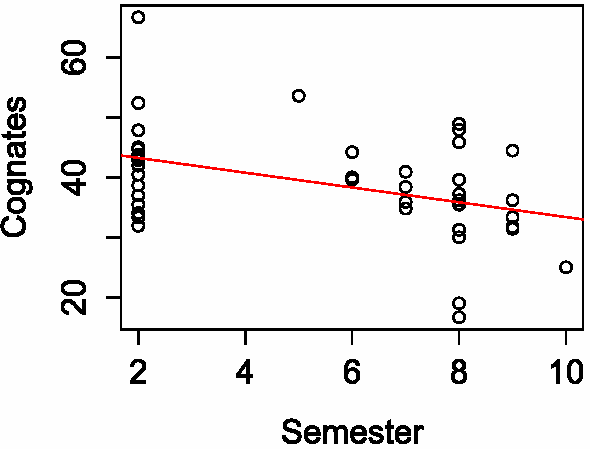
\includegraphics[width=0.6\textwidth]{figures/hansen-schirra/HansenSchirra8a.pdf}
\caption{Usage of cognate correlates with expertise}
\label{hansenschirraetal:fig:8}
\end{figure}

These results suggest that a mechanism in the translator's mind develops during the translator training. This could be the \isi{mental lexicon}, since it was shown that new words can also be easily learned in adulthood, and connections can be strengthened or weakened in its network-like structure \citep{Aitchison2012}. But the reason could also be due to increased monitoring (see \citealtv{Oster} for the impact of monitoring and \isi{mental lexicon} on the lexis of the target text). However, several studies concluded that monitoring does not develop anymore after childhood \citep{Wiersemaetal2007}. It depends, however, on the mental resources available: motivation \citep{GanushchakSchiller2008} and \isi{time pressure} \citep{GanushchakSchiller2006}.

Our hypothesis is thus that the \isi{mental lexicon} changes. It is reorganized; the connections between non-cognates become stronger since cognates are constantly filtered out by the monitoring process. Monitoring itself does not change. But as the translator needs less mental resources to activate non-cognates (their threshold is lowered over time), more mental resources are available for monitoring. This means that monitoring becomes stronger in translation tasks but not in general settings. We have to keep in mind, however, that the results might not only be due to the translator training but also to increased expertise in the respective languages. This expertise goes hand in hand with the expertise in translation. But it could be worth investigating this factor in future studies.

\subsection{Computer-aided translation}\label{hansenschirraetal:sec:4.2}
In the last decades, translation technologies have become more and more important as they make translations more consistent and the process more efficient. Translation memory systems and software for terminology management have been developed and established in most translation environments. A recent trend is the post-\isi{editing} of a machine translated source text ``by a human translator according to specific guidelines and quality criteria''. \citep[197]{OBrien2011} In this study, we hypothesize that the processing mode in which the translation is produced influences \isi{cognate} use. We therefore compare human translation output and post-edited output. We hypothesize that \isi{machine translation} generates more \isi{cognate} translations and that the translator tends to adhere to the \isi{machine translation}.

The experiments are part of the \textsc{critt-tpr} database\footnote{\url{https://sites.google.com/site/centretranslationinnovation/tpr-db}, last accessed 13th August 2016} that collects \isi{translation process} data for different tasks and in different languages. A total of 24 participants took part in the study used for this analysis: twelve professional and twelve \isi{semi-professional} translators (students of the university with only little professional work experience). The texts were newspaper articles and sociology-related texts with different complexity levels. The length of the texts varies between 100 and 148 words. The participants were asked to translate two texts from scratch, post-edit two machine translated texts and monolingually edit two machine translated texts – from English to \ili{German} respectively. For this study, we only looked at the post-edited and human translated target texts.

The tasks were conducted in Translog II,\footnote{\url{https://sites.google.com/site/centretranslationinnovation/translog-ii} last accessed 13th August 2016}, a program used for recording mouse activity, key strokes and gaze data with the help of the Tobii eye-tracker, which also records the sessions, mouse activity, key-strokes and gaze data in Tobii Studio. There were no time restrictions and the participants could use the Internet freely as a research tool.

We determined the cognates from the source texts (58 cognates in all six source texts – some occurred more than once in one text or in a few texts) and extracted the realizations of these cognates in the MT output and in the target texts (human translation and post-\isi{editing}). We differentiated between non-\isi{cognate} and \isi{cognate} translations. Further, we analyzed the varieties in the \isi{cognate} realizations in the different translation modes.

\tabref{hansenschirraetal:tab:3} and \ref{hansenschirraetal:tab:4} present the results of the \isi{cognate} analysis. While \tabref{hansenschirraetal:tab:3} presents total numbers (e. g. 321 cognates were realized with a \isi{cognate translation} in the translation from scratch mode), \tabref{hansenschirraetal:tab:4} shows the amount of variation in the different translations modes, independent of how often they occurred. Let us specify the counting procedure for \tabref{hansenschirraetal:tab:4} with some examples:

\begin{itemize}
\item The English \isi{cognate} \textit{motive} was realized as \textit{Motiv} both in the translation from scratch and in the post-\isi{editing} tasks. Hence, it was counted as TfS – Cognate: 1; TfS – Non-Cognate: 0; PE – Cognate: 1; PE – Non-Cognate: 0.
\item The \isi{cognate} \textit{minimized} was realized as \textit{minimieren}, \textit{reduzieren}, \textit{gering halten}, and \textit{verringern} in the translation from scratch tasks and as \textit{Minimie\-rung}, \textit{minimeren}, \textit{Reduzierung}, and \textit{Reduktion} in the post-\isi{editing} tasks. It was counted as TfS – Cognate: 1; TfS – Non-Cognate: 3; PE – Cognate: 2; PE – Non-Cognate: 2.
\item The \isi{cognate} \textit{analysts} was realized as \textit{Analysten}, \textit{Analytiker}, \textit{Analysen}, and \textit{Finanzexperten} in the translation from scratch tasks and as \textit{Analysten} and \textit{Experten} in the post-\isi{editing} tasks. It was counted as TfS – Cognate: 3; TfS – Non-Cognate: 1; PE – Cognate: 1; PE – Non-Cognate: 1.
\end{itemize}

\begin{table}
\caption{Translation of Cognates in translation from scratch (TfS) and post-editing (PE) task.}
\label{hansenschirraetal:tab:3}
\begin{tabularx}{.8\linewidth}{Xrr}
\lsptoprule
            & Cognate     & Non-Cognate \\ \midrule
TfS & 321 & 127 \\
PE & 325 & 118 \\
\lspbottomrule
\end{tabularx}
\end{table}

\begin{table}
\caption{Variations in translation from scratch (TfS) and post-editing (PE) task}
\label{hansenschirraetal:tab:4}
\begin{tabularx}{.8\linewidth}{Xrr}
\lsptoprule
    & Cognate & Non-Cognate \\ \midrule
TfS & 59 & 91 \\
PE & 50 & 49 \\ 
\lspbottomrule
\end{tabularx}
\end{table}


\tabref{hansenschirraetal:tab:3} shows that the distribution of English cognates realized as the \ili{German} cognate-equivalent is quite similar in both translation modes: 71.7\% in the translation from scratch task and 73.4\% in the post-\isi{editing} task. The chi-square test did not show significant differences between the two translation modes and the \isi{cognate} realization: $\chi^{2} = 0.2471, df = 1, p = 0.62$.

In the next step, we examined the variety in which the cognates were translated. While \isi{cognate} variety is quite similar, the difference is remarkable in non-\isi{cognate} variety. For the whole set-up, the chi-square test did not prove significance between the two translation modes and \isi{cognate} realization: $\chi^{2}=2.59, df=1, p=0.11$. Next, we conducted Wilcoxon rank sum tests (the data was not distributed normally) for the differences in the variation in the \isi{cognate} group and in the non-\isi{cognate} group. The test did not prove significant for the \isi{cognate} group ($W=1883, p=0.19$), but significant for the non-\isi{cognate} group ($W=2157.5, p=0.005$).

Translations from scratch and post-edited target texts show a similar \isi{cognate} and non-\isi{cognate} usage, which is not in line with our hypothesis. By implication, this indicates that post-\isi{editing} and human translation are very similar in this aspect. The machine translated \isi{cognate} was not changed in 88.3\% of instances (391 of 443) in the post-\isi{editing} task. Interestingly, 67.9\% (301 of 443) of the human translated cognates were congruent with the \isi{machine translation} output. Hence, we assume that \isi{cognate}/non-\isi{cognate} translations are chosen in statistical MT system quite similar to human translation. The variety within non-\isi{cognate} choices, however, is statistically higher in translations from scratch than in post-edited texts. When we take a closer look at the data, it turns out that the participants choose the MT in 87\%of cases, and only 11\% changed the MT. This explains why there is much more variety in human translations than in post-\isi{editing}.

\section{Enhancing the monitor model with translation predictors}\label{hansenschirraetal:sec:5}
The predictors presented in this study are not exclusive. Other translation-in\-her\-ent constraints that influence the usage of cognates in translation can be skopos, time constraints, translation mode \citepv{Oster,Gieshoff}, etc.

\newpage
The results suggest that different mechanisms are responsible for the translation of cognates. When considering, for example, Levelt’s \isi{speech production} model \citeyearpar{Levelt1989} as a basis for the processing of language during translation, the translation of words in general can be influenced by different steps. During the conceptualization phase, speakers adapt messages according to cultural and pragmatic norms. During formulation, the lexical selection in the \isi{mental lexicon} can be primed by context and can depend on expertise.

When considering the translation of cognates, we can assume that according to the \isi{literal translation} hypothesis (Halverson 2015), the translator always chooses the easiest path (the \isi{cognate translation}). However, when considering cultural predictors for \isi{cognate translation}, specific cultural norms are present at a translator’s conceptual level causing monitoring \citep{TirkkonenCondit2005}. The same holds true for pragmatics. On a lexical level, the context pre-activates certain words (cognates or non-cognates). It causes thus less processing effort for the translator to choose the co-activated words than to look for alternatives. The mechanisms of controlling lexical choices might change with expertise according to \citet{Halverson2015} gravitational pull hypothesis and thus lead to more pre-activation of non-cognates in experienced translators.

The findings related to the translation of cognates suggest that different priming roots exist and that the \isi{monitor model} proposed by Tirkkonen-Condit should be adapted to these findings. The studies we presented are, however, pilot studies which were conducted in very natural settings. If we want to further explore the predictors of translations, we will need to conduct more controlled experiments in order to isolate different factors. However, the studies we presented in this paper can provide an overview of the different processes that might be involved. Future research might also consider other linguistic aspects such as syntax or pragmatics, and investigate how these features can be influenced by different conditions. This might help us to predict how a certain translator will translate a text in a certain situation.

\sloppy
\printbibliography[heading=subbibliography,notkeyword=this]
\end{document}
